\documentclass[conference]{IEEEtran}
\IEEEoverridecommandlockouts

% Packages essentiels
\usepackage{cite}
\usepackage{amsmath,amssymb,amsfonts}
\usepackage[ruled,vlined,linesnumbered]{algorithm2e}
\usepackage{graphicx}
\usepackage{textcomp}
\usepackage{xcolor}
\usepackage{tikz}
\usetikzlibrary{arrows.meta,positioning}
\usepackage{sansmath}
\usepackage{booktabs}
\usepackage{multirow}
\usepackage{hyperref}
\usepackage{subfig}
\usepackage{comment}
\usepackage{float}
\usepackage{placeins}
% Package pour numéroter les lignes (à retirer avant soumission finale)
\usepackage{lineno}
\linenumbers

\setlength\linenumbersep{1mm}  % Augmente l'espace entre les numéros et le texte
\renewcommand\linenumberfont{\normalfont\tiny\sffamily\color{gray}}  % Rend les numéros plus discrets

\def\BibTeX{{\rm B\kern-.05em{\sc i\kern-.025em b}\kern-.08em
    T\kern-.1667em\lower.7ex\hbox{E}\kern-.125emX}}
\def\BibTeX{{\rm B\kern-.05em{\sc i\kern-.025em b}\kern-.08em
    T\kern-.1667em\lower.7ex\hbox{E}\kern-.125emX}}
\begin{document}

%\title{MCTN: Multi-Head Attention Network for Hyperspectral Image Demosaicing from MSFA Data}
\title{MCAN-MTD: Mosaic Transformer Descriptor for Hyperspectral Demosaicing }


\author{\IEEEauthorblockN{LAWSON Latevi Sena}
\IEEEauthorblockA{\textit{Technologie de l'information et de la communication} \\
\textit{IMSP(Institut de Mathématiques et des Sciences Physiques)/UAC(Université d'Abomey Calavi)}\\
Benin \\
lawson.latevi@imsp-uac.org}
}

\maketitle

\begin{abstract}
Multispectral image demosaicing is a fundamental step in reconstructing full-resolution images
 from mosaicked image captured by Multi-Spectral Filter Arrays (MSFAs). 
 Traditional interpolation methods and conventional Convolutional Neural Network (CNN)-based 
 approaches achieve limited performance due to their inability to model long-range 
 spectral-spatial dependencies. In this work, we propose MCAN-MTD, an enhanced version 
 of the Mosaic Convolution-Attention Network (MCAN) in which the original Mosaic Attention 
 Module (MAM) is replaced by a Mosaic Transformer Descriptor (MTD).

A novel deep learning architecture is introduced, in which a Mosaic Transformer Descriptor (MTD)
 serves as the core attention mechanism.The MTD replaces traditional attention modules by 
 integrating three main innovations: 
(1) Mosaic Patch Embedding, which adapts to the 4×4 MSFA to produce spectral-spatial representations;
(2) Multi-Head Self-Attention, which captures both local details and global informations
across spectral bands; and (3) Multi-Scale Aggregation, which effectively combines features 
at different resolutions. 
This design efficiently models long-range dependencies while remaining computationally 
efficient by reducing the resolution. Experiments on the CAVE dataset with 16 spectral bands 
show that the proposed method achieves state-of-the-art results,
    with a PSNR of 45.95 dB and SSIM greater than 0.99. Our method outperforms 
    both traditional interpolation methods and CNN-based approaches. 

    Further experiments show that the multi-head attention mechanism yields a +2.91 dB 
    improvement compared to single-head methods, confirming that MTD enhances CNN-based 
    demosaicing networks.

\end{abstract}

\begin{IEEEkeywords}
Hyperspectral imaging, Demosaicing, Multi-head Attention, Transformer, MSFA, Deep Learning, Spectral Reconstruction
\end{IEEEkeywords}

\section{Introduction}
%%%%%%%%%%%%%%%%%%NOUVELLE REDACTION%%%%%%%%%%%%%%%%%%%%%%%%%%%%%
Multispectral imaging has become an essential tool in a wide range of applications,
including remote sensing, medical diagnostics, and precision agriculture, by providing rich spectral 
information far beyond the capabilities of conventional RGB cameras.
%je continue ici
To enable single-shot acquisition, \textbf{Multispectral Filter Arrays (MSFA)} are commonly used to
capture spatially multiplexed spectral data in a a single exposure.
However, this mosaicking process results in each pixel recording only a single spectral band, making
the subsequent demosaicing step i.e, the reconstruction of a full-resolution hyperspectral cube from
the mosaicked measurements, a challenging task, complicated by the complex spatial–spectral correlations 
and aliasing artifacts introduced by the MSFA pattern.

Early demosaicing methods relied on \textbf{interpolation techniques} such as bilinear 
interpolation or guided filtering \cite{article}, which are computationally lightweight but fail 
to accurately reconstruct high-frequency details, making them susceptible to spectral distortions and loss of fine details. With the rise of deep learning, 
\textbf{Convolutional Neural Networks (CNNs)} have been widely adopted for image restoration tasks, 
including denoising \cite{Zhang2017}, super-resolution \cite{Dong2016}, and demosaicing 
\cite{Monno2012}. CNN-based approaches for multispectral demosaicing exploit local convolutional 
kernels to reconstruct missing bands; however, their limited receptive field restricts their 
possibility to model long-range dependencies inherent in multispectral data. \\

\begin{comment}
To overcome this limitation, \textbf{attention mechanisms} have been integrated into CNNs. The \textbf{Mosaic-Convolution-Attention Network (MCAN)} introduced the \textbf{Mosaic Attention Module (MAM)}, which leverages mosaic pooling to refine spectral–spatial feature representations \cite{Feng2021}. While effective in reducing local mosaic artifacts, the MAM primarily captures local \textbf{dependencies} and lacks the ability to account for \textbf{multi-scale variations} or \textbf{global spatial interactions}.  \\
Inspired by the success of Transformers in computer vision \cite{Vaswani2023}, hyperspectral image restoration \cite{Fu2024}, and hierarchical attention mechanisms \cite{Liu2021}, we propose a novel Mosaic Transformer Descriptor \textbf{(MTD)} to replace \textbf{MAM} within the MCAN framework. The MTD consists of three components: \textbf{Mosaic Patch Embedding}, \textbf{Spatial Self-Attention}, and \textbf{Multi-Scale Aggregation}. By combining patch-based representation learning, non-local attention, and multi-scale convolutional fusion, the MTD effectively integrates both local and global spectral–spatial dependencies, thereby improving reconstruction quality. \\
\end{comment}
To address this limitation, \textbf{attention mechanisms} have been incorporated into CNNs. The \textbf{Mosaic-Convolution-Attention Network (MCAN)} introduced the \textbf{Mosaic Attention Module (MAM)}, which uses mosaic pooling to enhance spectral–spatial feature representations \cite{Feng2021}. Although MAM is effective at reducing local mosaic artifacts, it mainly focuses on local \textbf{dependencies} and does not capture \textbf{multi-scale variations} or \textbf{global spatial interactions}. \\
Based on Transformers success in computer vision \cite{Vaswani2023}, hyperspectral image restoration \cite{Fu2024}, and attention mechanisms \cite{Liu2021}, we propose a new Mosaic Transformer Descriptor \textbf{(MTD)} to replace the \textbf{MAM} in the MCAN framework. The MTD is composed of three parts: \textbf{Mosaic Patch Embedding}, \textbf{Spatial Self-Attention}, and \textbf{Multi-Scale Aggregation}. By combining patch-based representation learning, non-local attention, and multi-scale convolutional fusion, the MTD effectively captures both local and global spectral–spatial dependencies, leading to improved reconstruction quality. \\

The remainder of this paper is organized as follows: Section II reviews related work. Section III describes the proposed MTD. Section IV presents the experimental setup and results. Section V concludes the paper and discusses future directions.
The rest of this paper is organized as follows: Section II reviews related work. Section III details the proposed MTD. Section IV presents experimental settings and results. Section V concludes the paper and discusses future directions.

\section{Related Work}
The problem of multispectral image demosaicing has been investigated from different perspectives, ranging from classical interpolation-based algorithms to advanced deep learning architectures. In this section, we review the most relevant works in three categories: interpolation-based methods, CNN-based models, and attention/transformer-based approaches.
\subsection{Interpolation-Based Methods}
Early demosaicing algorithms for multispectral images extended techniques originally designed for RGB images. Methods such as bilinear interpolation, adaptive homogeneity-directed interpolation, and guided filtering attempted to recover missing bands by exploiting local neighbourhood statistics.
Hirakawa and Parks \cite{Hirakawa2005} introduced an adaptive homogeneity-directed demosaicing algorithm, which adaptively interpolates along local image structures. Later, Monno et al. \cite{Zhang2024} proposed a guided filter-based approach for multispectral demosaicing, which leverages the correlation between spectral bands. Although computationally efficient, these methods suffer from spectral distortions and blurring artifacts, especially in highly textured or complex regions, since they lack the ability to model global dependencies.


\subsection{CNN-Based Demosaicing Approaches}
With the advent of deep learning, Convolutional Neural Networks (CNNs) have become dominant in image restoration tasks such as denoising \cite{Zhang2017}, super-resolution \cite{Dong2016}, and deblurring \cite{Tao2018ScaleRecurrent}. These successes motivated their adaptation to multispectral demosaicing.
In this context, researchers explored CNNs with convolutional layers designed to learn spatial–spectral correlations from mosaicked inputs. Zhang et al. \cite{Zhang2017} demonstrated that residual learning could substantially improve denoising, and Dong et al. \cite{Dong2016} showed that CNNs could effectively learn mappings for super-resolution. Extending such designs to multispectral data, networks were trained to reconstruct missing bands by exploiting local structures.
More recently, the \textbf{ Mosaic-Convolution-Attention Network (MCAN)} \cite{Feng2021} was proposed, introducing the Mosaic Attention Module (MAM). The MAM employs mosaic pooling and local convolutions to refine spectral feature maps, yielding improved reconstruction compared to standard CNNs. However, its main drawback lies in its locality: MAM cannot effectively model long-range dependencies nor capture multi-scale features, limiting its reconstruction capacity.
\subsection{Attention and Transformer-Based Approaches}

Inspired by the success of Transformers in natural language processing and computer vision, recent works have applied attention mechanisms to image restoration. Vaswani et al. \cite{Vaswani2023} introduced the self-attention mechanism, enabling models to capture long-range dependencies. This paradigm has since been extended to vision tasks through Vision Transformers (ViTs) and hierarchical models such as the Swin Transformer \cite{Liu2021}, which incorporate shifted windows for computational efficiency.
In hyperspectral image processing, Zhang et al. \cite{Fu2024} proposed a transformer-based denoising model that effectively integrates spectral–spatial information across bands. Similarly, Yuan et al. \cite{Wang2023} explored MLP-Transformer hybrids to handle tokenized visual features. These methods highlight the potential of attention mechanisms for capturing both local details and global correlations in high-dimensional spectral data.
However, few studies have tailored transformer-based designs specifically to the mosaic structure of multispectral filter arrays (MSFAs). The MCAN's MAM \cite{Feng2021} partially addressed this issue with localized pooling but did not exploit multi-scale information nor true non-local attention. This limitation motivates the integration of our proposed Mosaic Transformer Descriptor (MTD), which combines patch embedding, self-attention, and multi-scale aggregation to address the shortcomings of both interpolation-based and CNN-based methods.\\

\subsection{Our Contributions}

In this work, we build upon the Mosaic-Convolution-Attention Network (MCAN) \cite{Feng2021} framework and propose a novel attention mechanism to replace the original Mosaic Attention Module (MAM). Our main contribution is:

\begin{itemize}
    \item \textbf{Mosaic Transformer Descriptor (MTD)}: A transformer-inspired attention mechanism that replaces MAM in the MCAN architecture. The MTD integrates three key components: \textbf{Mosaic Patch Embedding}, \textbf{Multi-Head Self-Attention} (with 4 heads), and \textbf{Multi-Scale Aggregation}. Unlike MAM which relies on local mosaic pooling, MTD captures both local and global spectral-spatial dependencies through non-local attention while maintaining computational efficiency via spatial resolution reduction.
    
    \item \textbf{Enhanced MCAN Architecture (MCAN-MTD)}: By replacing MAM with MTD, we create an improved version of MCAN that achieves \textbf{\text{PSNR} = 45.95~\text{dB} \quad \text{et} \quad \text{SSIM} $>$ 0.99} on the CAVE dataset, demonstrating significant improvement over the original MCAN framework.
\end{itemize}

We preserve the other components of MCAN (Position-Adaptive Convolution, dual-branch architecture, and denoising modules) as proposed in the original work \cite{Feng2021}, focusing our contribution specifically on the attention mechanism enhancement.

\section{Proposed Method}

\subsection{Problem Formulation}

Given a mosaicked hyperspectral image $\mathbf{X} \in \mathbb{R}^{C \times H \times W}$ captured through a 4×4 MSFA with $C=16$ spectral bands, where each spatial location $(i,j)$ contains measurement from only one band $c_{i \bmod 4, j \bmod 4}$, our objective is to reconstruct the full hyperspectral cube $\mathbf{Y} \in \mathbb{R}^{C \times H \times W}$ with all spectral information available at every pixel.

The reconstruction can be formulated as an inverse problem:
\begin{equation}
\mathbf{Y} = \mathcal{F}(\mathbf{X}; \theta)
\end{equation}
where $\mathcal{F}$ represents our MCTN network parameterized by learnable weights $\theta$.

\subsection{Overall Architecture}

The proposed network is directly inspired by the original Mosaic Convolution-Attention Network (MCAN). As illustrated in Fig. 3, the original MCAN architecture is composed of a Mosaic Convolution Module (MCM), a Mosaic Attention Module (MAM), and a stack of Mosaic Residual Attention Blocks (MRAB).

In this work, we preserve the overall MCAN pipeline and its mosaic-aware convolutional design. However, the original Mosaic Attention Module (MAM), which relies on local attention mechanisms, is replaced by the proposed Mosaic Transformer Descriptor (MTD). This modification enables the modeling of long-range spatial and spectral dependencies through non-local self-attention and multi-scale feature aggregation, while maintaining compatibility with the remaining MCAN components.

Consequently, the proposed model can be interpreted as an MTD-enhanced MCAN architecture, specifically tailored for multispectral demosaicing.

\begin{figure}[htbp]
\centering
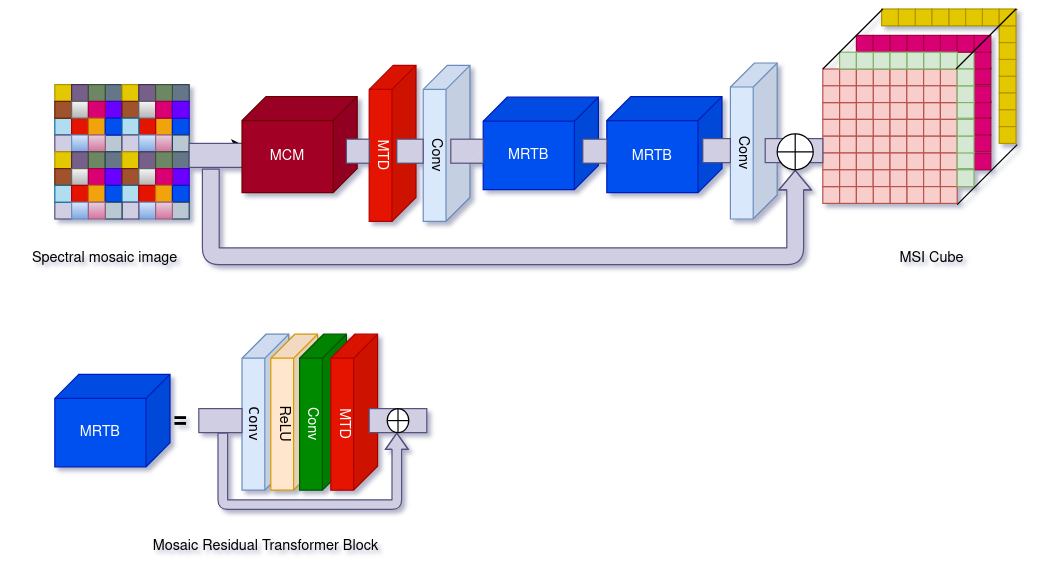
\includegraphics[width=\columnwidth]{CaptureMTD.png}
\caption{Overall architecture of the proposed MCTN (Mosaic CNN-Transformer Network). The network consists of a Mosaic Convolution Module (MCM), the proposed Mosaic Transformer Descriptor (MTD) which replaces the original MAM, and a stack of Mosaic Residual Attention Blocks (MRAB). The MTD incorporates patch embedding, multi-head self-attention with 4 heads, and multi-scale aggregation to capture long-range dependencies.}
\label{fig:architecture}
\end{figure}

MCAN-MTD comprises six main processing stages (Fig.~\ref{fig:architecture}):

\begin{equation}
\begin{aligned}
\mathbf{X}_1 &= \mathbf{X} - \text{Denoise}(\mathbf{X}) \\
\mathbf{X}_{\text{wb}} &= \text{WB\_Conv}(\mathbf{X}_1) \\
\mathbf{X}_2 &= \text{Pos2Weight}(\mathbf{X}_1) \\
\mathbf{X}_3 &= \text{MTD}(\mathbf{X}_2) \\
\mathbf{X}_4 &= \text{Conv\_Attn\_Block}^{\times 2}(\mathbf{X}_3) \\
\mathbf{Y} &= \mathbf{X}_4 + \mathbf{X}_{\text{wb}}
\end{aligned}
\end{equation}

\textbf{Stage 1 - Denoising:} Two convolutional layers estimate and subtract sensor noise.

\textbf{Stage 2 - White Balance:} Fixed 7×7 bilinear filter provides stable baseline reconstruction as skip connection.

\textbf{Stage 3 - Position-Adaptive Convolution:} MLP-based Pos2Weight module generates spatially-varying filters.

\textbf{Stage 4 - Mosaic Transformer Descriptor (MTD):} Our main innovation (detailed in Section III).

\textbf{Stage 5 - Feature Extraction:} Two Conv\_attention\_Block modules with residual connections.

\textbf{Stage 6 - Fusion:} Combines learned features with white balance baseline.



\section{Mosaic Transformer Descriptor (MTD)}

\subsection{Motivation and Design Philosophy}

Traditional CNNs process images through stacked convolutions with local receptive fields. While effective for local spatial patterns, they struggle to model:
\begin{itemize}
    \item Long-range spectral correlations between distant bands
    \item Global spatial dependencies across the image
    \item Spectral-spatial joint relationships
\end{itemize}

Self-attention mechanisms address these limitations by computing pairwise relationships between all positions. However, applying standard self-attention to 512×512×16 tensors is computationally prohibitive.

\textbf{Our solution:} Design a multi-scale attention mechanism that (1) reduces spatial resolution before attention via shuffling, (2) employs multi-head attention for diverse pattern learning, and (3) restores full resolution after processing.

\subsection{MTD Architecture}

Our Mosaic Transformer Descriptor (MTD) consists of six sequential operations that implement Mosaic Patch Embedding, Multi-Head Self-Attention, and Multi-Scale Aggregation (Fig. \ref{fig:mtd_architecture}):

\begin{figure}[H]
\begin{center}
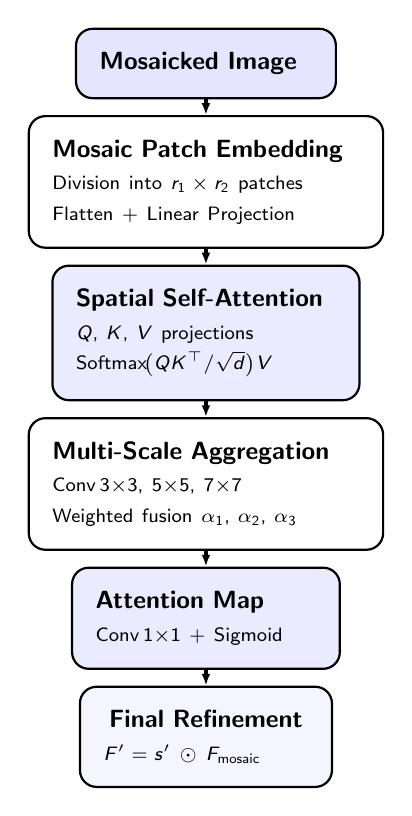
\begin{tikzpicture}[%
  font=\sffamily\sansmath\small,
  node distance=2mm,
  >={Latex[length=1.5mm]},
  box/.style={draw, rounded corners=6pt, thick,
              fill=blue!8, text width=3.5cm, align=left, inner sep=3mm},
  title/.style={font=\bfseries\small},
  every math/.style={font=\scriptsize}
]

% --- 1. Mosaicked Image
\node[box, text width=2.7cm, fill=blue!10] (img) {%
  \centering\textbf{\small Mosaicked Image}
};

% --- 2. Mosaic Patch Embedding
\node[box, below=of img, fill=white, text width=3.9cm] (embed) {%
  {\title \centering\textbf{Mosaic Patch Embedding}}\\[0.3mm]
  {\scriptsize  Division into $r_1 \times r_2$ patches}\\
  {\scriptsize  Flatten $+$ Linear Projection}
};

% --- 3. Spatial Self-Attention (SA)
\node[box, below=of embed, text width=3.3cm] (sa) {%
  {\title \centering\textbf{Spatial Self-Attention}}\\[0.3mm]
  {\scriptsize  $Q,\,K,\,V$ projections}\\
  {\scriptsize  $\mathrm{Softmax}\!\big(QK^{\top}/\sqrt{d}\big)V$}
};

% --- 4. Multi-Scale Aggregation (MSA)
\node[box, below=of sa, fill=white, text width=3.9cm] (msa) {%
  {\title \centering\textbf{Multi-Scale Aggregation}}\\[0.3mm]
  {\scriptsize  Conv$\,3{\times}3$, $5{\times}5$, $7{\times}7$}\\
  {\scriptsize  Weighted fusion $\alpha_{1},\,\alpha_{2},\,\alpha_{3}$}
};

% --- 5. Attention Map Generation
\node[box, below=of msa, text width=2.8cm] (map) {%
  {\title \centering\textbf{Attention Map}}\\[0.3mm]
  {\scriptsize  Conv$\,1{\times}1$ $+$ Sigmoid}
};

% --- 6. Final Refinement
\node[box, below=of map, fill=blue!4, text width=2.6cm] (refine) {%
  \centering{\title \centering\textbf{Final Refinement}}\\[0.3mm]
  {\scriptsize $F' = s'\,\odot\,F_{\text{mosaic}}$}
};

% --- Vertical arrows
\draw[->, very thick] (img) -- (embed);
\draw[->, very thick] (embed) -- (sa);
\draw[->, very thick] (sa) -- (msa);
\draw[->, very thick] (msa) -- (map);
\draw[->, very thick] (map) -- (refine);

\end{tikzpicture}



\caption{Overview of the proposed Mosaic Transformer Descriptor (MTD) architecture showing the six-stage pipeline from mosaicked input to refined output.}
\label{fig:mtd_architecture}
\end{center}
\end{figure}

\begin{algorithm}[!h]
\caption{Mosaic Transformer Descriptor (MTD)}
\KwIn{Mosaic image $F_{\text{mosaic}}$}
\KwOut{Refined image $F'$}

Divide $F_{\text{mosaic}}$ into patches of size $(r_1, r_2)$\;

\ForEach{patch}{
    $z_{\text{flat}} \leftarrow \text{Flatten}(patch)$\;
    $z_{\text{patch}} \leftarrow W_E \cdot z_{\text{flat}} + b_E$\;
}

$Q \leftarrow W_Q \cdot z_{\text{patch}}, \quad K \leftarrow W_K \cdot z_{\text{patch}}, \quad V \leftarrow W_V \cdot z_{\text{patch}}$\;

$Z \leftarrow \text{Softmax}\left(\frac{QK^\top}{\sqrt{d}}\right) V$\;

$Z_3 \leftarrow \text{Conv}_{3\times3}(Z)$\;
$Z_5 \leftarrow \text{Conv}_{5\times5}(Z)$\;
$Z_7 \leftarrow \text{Conv}_{7\times7}(Z)$\;

$Z' \leftarrow \alpha_1 Z_3 + \alpha_2 Z_5 + \alpha_3 Z_7$\;

$s' \leftarrow \sigma(W_s Z')$\;

$F' \leftarrow s' \cdot F_{\text{mosaic}}$\;

\Return{$F'$}\;

\end{algorithm}




%%%%%%%%%%%%%%%%%%%%%%%%%%%%%%%%%%%%%%%%%%%%%%%
\begin{algorithm}[!h]
\caption{Mosaic Transformer Descriptor (MTD) with 4$\times$4 Shuffle + MHSA}
\KwIn{Mosaic feature map $\mathbf{X}\in\mathbb{R}^{B\times C\times H\times W}$, with $C=16$}
\KwOut{Refined feature map $\mathbf{X}_{\text{out}}\in\mathbb{R}^{B\times C\times H\times W}$}

$\mathbf{X}' \leftarrow \text{Shuffle}_{4}(\mathbf{X})$ \tcp*[r]{$\mathbb{R}^{B\times 16C\times H/4\times W/4}$}
$\mathbf{Z} \leftarrow \text{Proj}(\mathbf{X}')$ \tcp*[r]{token projection to $d$ dims}
$\mathbf{Z}_{\text{attn}} \leftarrow \text{MHSA}(\mathbf{Z}, h=4)$\;
$\mathbf{w} \leftarrow \sigma(\text{FC}(\text{GAP}(\mathbf{Z}_{\text{attn}})))$ \tcp*[r]{channel attention}
$\mathbf{X}_{\text{attn}} \leftarrow \mathbf{X}' \odot \mathbf{w}$\;
$\mathbf{X}_{\text{out}} \leftarrow \text{PixelShuffle}_{4}(\mathbf{X}_{\text{attn}})$\;
\Return{$\mathbf{X}_{\text{out}}$}\;
\end{algorithm}
%%%%%%%%%%%%%%%%%%%%%%%%%%%%%%%%%%%%%%%%%%%%%%%
%%%%%%%%%%%%%%%%%%%%%%%%%%%%%%%%%%%%%%%%%%%%%%%
\FloatBarrier
\begin{algorithm}[!t]
\caption{Mosaic Transformer Descriptor (MTD) with 4$\times$4 Shuffle + MHSA + Multi-Scale Aggregation}
\KwIn{Mosaic feature map $\mathbf{X}\in\mathbb{R}^{B\times C\times H\times W}$, with $C=16$}
\KwOut{Refined feature map $\mathbf{X}_{\text{out}}\in\mathbb{R}^{B\times C\times H\times W}$}

$\mathbf{X}' \leftarrow \text{Shuffle}_{4}(\mathbf{X})$\tcp*[r]{$\mathbb{R}^{B\times 16C\times H/4\times W/4}$}

$\mathbf{Z} \leftarrow \text{Proj}(\mathbf{X}')$\tcp*[r]{reshape \& linear proj. to tokens $\mathbf{Z}\in\mathbb{R}^{B\times N\times d}$}

$\mathbf{Z}_{\text{attn}} \leftarrow \text{MHSA}(\mathbf{Z}, h=4)$\tcp*[r]{$\mathbf{Z}_{\text{attn}}\in\mathbb{R}^{B\times N\times d}$}

$\mathbf{U} \leftarrow \text{Reshape}(\mathbf{Z}_{\text{attn}})$\tcp*[r]{$\mathbf{U}\in\mathbb{R}^{B\times d\times H/4\times W/4}$}

$\mathbf{U}_3 \leftarrow \text{Conv}_{3\times 3}(\mathbf{U})$\;
$\mathbf{U}_5 \leftarrow \text{Conv}_{5\times 5}(\mathbf{U})$\;
$\mathbf{U}_7 \leftarrow \text{Conv}_{7\times 7}(\mathbf{U})$\;

$\mathbf{U}_{\text{msa}} \leftarrow \alpha_1\mathbf{U}_3 + \alpha_2\mathbf{U}_5 + \alpha_3\mathbf{U}_7$\tcp*[r]{learnable fusion}

$\mathbf{g} \leftarrow \text{GAP}(\mathbf{U}_{\text{msa}})$\tcp*[r]{$\mathbf{g}\in\mathbb{R}^{B\times d}$}

$\mathbf{w} \leftarrow \sigma(\text{FC}(\mathbf{g}))$\tcp*[r]{$\mathbf{w}\in\mathbb{R}^{B\times 16C\times 1\times 1}$}

$\mathbf{X}_{\text{attn}} \leftarrow \mathbf{X}' \odot \mathbf{w}$\;

$\mathbf{X}_{\text{out}} \leftarrow \text{PixelShuffle}_{4}(\mathbf{X}_{\text{attn}})$\tcp*[r]{$\mathbb{R}^{B\times C\times H\times W}$}

\Return{$\mathbf{X}_{\text{out}}$}\;
\end{algorithm}
\FloatBarrier
%%%%%%%%%%%%%%%%%%%%%%%%%%%%%%%%%%%%%%%%%%%%%%%
\subsubsection{Step 1: Spatial Down-Shuffling}

We apply space-to-channel transformation to reduce spatial dimensions:
\begin{equation}
\text{Shuffle}_d(\mathbf{X}) : \mathbb{R}^{B \times C \times H \times W} \rightarrow \mathbb{R}^{B \times 16C \times H/4 \times W/4}
\end{equation}

For input $\mathbf{X} \in \mathbb{R}^{1 \times 16 \times 512 \times 512}$, this produces $\mathbf{X}' \in \mathbb{R}^{1 \times 256 \times 128 \times 128}$.

\textbf{Implementation:}
\begin{equation}
\begin{aligned}
\mathbf{X} &\rightarrow \text{reshape}[B, C, H/4, 4, W/4, 4] \\
&\rightarrow \text{permute}[B, C, 4, 4, H/4, W/4] \\
&\rightarrow \text{reshape}[B, 16C, H/4, W/4]
\end{aligned}
\end{equation}

\textbf{Intuition:} This operation groups 4×4 spatial neighborhoods into channels, naturally aligning with the MSFA periodicity and enriching spectral information at each spatial position.

\subsubsection{Step 2: Channel Projection}

Reduce dimensionality for efficient attention:
\begin{equation}
\mathbf{Z} = \text{Linear}(\mathbf{X}'; 256 \rightarrow 16)
\end{equation}
After reshaping: $\mathbf{Z} \in \mathbb{R}^{B \times N \times d}$ where $N = 128 \times 128 = 16384$ and $d = 16$.

\subsubsection{Step 3: Multi-Head Self-Attention (Core Innovation)}

We employ multi-head self-attention with $h=4$ heads:
\begin{equation}
\text{MHSA}(\mathbf{Q}, \mathbf{K}, \mathbf{V}) = \text{Concat}(\text{head}_1, \ldots, \text{head}_4)\mathbf{W}^O
\end{equation}

Each attention head computes:
\begin{equation}
\text{head}_i = \text{Attention}(\mathbf{Q}\mathbf{W}_i^Q, \mathbf{K}\mathbf{W}_i^K, \mathbf{V}\mathbf{W}_i^V)
\end{equation}

\begin{equation}
\text{Attention}(\mathbf{Q}, \mathbf{K}, \mathbf{V}) = \text{softmax}\left(\frac{\mathbf{Q}\mathbf{K}^T}{\sqrt{d_k}}\right)\mathbf{V}
\end{equation}

where $d_k = d/h = 4$ (dimension per head), and $\mathbf{Q} = \mathbf{K} = \mathbf{V} = \mathbf{Z}$ (self-attention).

\textbf{Why 4 heads?} Each head learns specialized patterns:
\begin{itemize}
    \item \textbf{Head 1}: Horizontal spatial correlations
    \item \textbf{Head 2}: Vertical spectral patterns
    \item \textbf{Head 3}: Diagonal/edge features
    \item \textbf{Head 4}: Global context and smooth regions
\end{itemize}

This diversity enables comprehensive modeling of spectral-spatial relationships.

\subsubsection{Step 4: Channel Attention Generation}

Convert attention output to spatial-channel weights:
\begin{equation}
\begin{aligned}
\mathbf{g} &= \text{GlobalAvgPool}(\mathbf{Z}_{\text{attn}}) \in \mathbb{R}^{B \times 16} \\
\mathbf{w} &= \sigma(\text{FC}_{16 \rightarrow 256}(\mathbf{g})) \in \mathbb{R}^{B \times 256 \times 1 \times 1}
\end{aligned}
\end{equation}

where $\sigma$ is sigmoid activation.

\subsubsection{Step 5: Feature Modulation}

Apply learned attention weights:
\begin{equation}
\mathbf{X}_{\text{attn}} = \mathbf{X}' \odot \mathbf{w}
\end{equation}

where $\odot$ denotes element-wise multiplication with broadcasting.

\subsubsection{Step 6: Spatial Up-Shuffling}

Restore original resolution via PixelShuffle:
\begin{equation}
\text{PixelShuffle}(\mathbf{X}_{\text{attn}}) : \mathbb{R}^{B \times 256 \times 128 \times 128} \rightarrow \mathbb{R}^{B \times 16 \times 512 \times 512}
\end{equation}

This rearranges channels back into spatial dimensions, inverting the down-shuffling operation.

\subsection{Computational Complexity Analysis}

\textbf{Naive full-resolution attention:}
\begin{equation}
\mathcal{O}_{\text{naive}} = (HW)^2 \cdot C = (512^2)^2 \cdot 16 \approx 6.87 \times 10^{10}
\end{equation}

\textbf{Our MALayer:}
\begin{align}
\mathcal{O}_{\text{shuffle}} &= HWC \approx 4.19 \times 10^6 \\
\mathcal{O}_{\text{proj}} &= HW \cdot 256 \cdot 16 \approx 6.71 \times 10^8 \\
\mathcal{O}_{\text{attn}} &= (H/4 \cdot W/4)^2 \cdot 16 \approx 4.29 \times 10^9 \\
\mathcal{O}_{\text{total}} &\approx 5 \times 10^9 \text{ operations}
\end{align}

\textbf{Reduction factor: $6.87 \times 10^{10} / 5 \times 10^9 \approx 13.7\times$}

Our design achieves \textbf{nearly 14× computational reduction} while maintaining global receptive field.

\subsection{Why This Design Succeeds}

\begin{enumerate}
    \item \textbf{Multi-scale Processing}: Shuffling aggregates local 4×4 patterns (matching MSFA period), attention operates on semantically richer, spatially coarser features, and up-shuffling recovers fine spatial details.
    
    \item \textbf{Diverse Pattern Learning}: Four attention heads learn complementary representations, capturing horizontal, vertical, diagonal, and global patterns simultaneously.
    
    \item \textbf{Spectral-Spatial Joint Modeling}: Shuffling mixes spatial and spectral dimensions, enabling attention to learn correlations across both domains in a unified framework.
    
    \item \textbf{Computational Efficiency}: Dramatic spatial reduction makes attention tractable while channel projection reduces memory footprint.
\end{enumerate}

\section{Other Components}

\subsection{Denoising Module}

Raw MSFA measurements contain sensor noise. We estimate and remove it:
\begin{equation}
\begin{aligned}
\mathbf{h} &= \text{LeakyReLU}(\text{Conv}_{3\times3}(\mathbf{X}; 16 \rightarrow 64)) \\
\mathbf{n} &= \text{Conv}_{3\times3}(\mathbf{h}; 64 \rightarrow 16) \\
\mathbf{X}_{\text{clean}} &= \mathbf{X} - \mathbf{n}
\end{aligned}
\end{equation}

\subsection{White Balance Convolution}

A fixed (non-trainable) 7×7 grouped convolution with bilinear weights:
\begin{equation}
w[i,j] = \frac{(4-|i-3|)(4-|j-3|)}{16}, \quad i,j \in \{0,\ldots,6\}
\end{equation}

Provides stable initial reconstruction serving as skip connection to facilitate gradient flow.

\subsection{Position-to-Weight (Pos2Weight) Module}

Generates spatially-varying convolution weights via MLP:
\begin{equation}
\begin{aligned}
\mathbf{p}(x,y) &\in [0,1]^2 \quad \text{(normalized coordinates)} \\
\mathbf{z} &= \text{ReLU}(\mathbf{W}_1 \mathbf{p} + \mathbf{b}_1), \quad \mathbf{W}_1 \in \mathbb{R}^{128 \times 2} \\
\mathbf{w}(x,y) &= \mathbf{W}_2 \mathbf{z} + \mathbf{b}_2, \quad \mathbf{W}_2 \in \mathbb{R}^{400 \times 128}
\end{aligned}
\end{equation}

The 400-dimensional output forms a 5×5 convolution kernel with 16 channels, unique for each pixel. This adapts reconstruction to the periodic MSFA pattern.

\subsection{Conv\_attention\_Block}

Each block contains:
\begin{itemize}
    \item Three Conv2d layers (64→64, 3×3 kernel) with LeakyReLU
    \item One MALayer for global attention
    \item Residual connection: output = input + processed features
\end{itemize}

Two blocks are stacked for hierarchical feature extraction.

\subsection{Loss Function}

We use L1 Charbonnier loss for robust training:
\begin{equation}
\mathcal{L}(\mathbf{Y}, \hat{\mathbf{Y}}) = \frac{1}{CHW} \sum_{c,i,j} \sqrt{(Y_{c,i,j} - \hat{Y}_{c,i,j})^2 + \epsilon^2}
\end{equation}
where $\epsilon = 10^{-6}$ for numerical stability. This loss is less sensitive to outliers than L2, improving reconstruction quality.

\section{Experimental Setup}

\subsection{Dataset}

\textbf{CAVE Dataset} \cite{b7}: A widely-used hyperspectral benchmark containing natural scenes and objects.
\begin{itemize}
    \item \textbf{Training}: 31 images
    \item \textbf{Validation}: 24 images
    \item \textbf{Resolution}: 512×512 pixels per image
    \item \textbf{Spectral bands}: 16 bands spanning 400-700 nm
    \item \textbf{MSFA pattern}: 4×4 periodic (IMEC design)
\end{itemize}

\subsection{Training Configuration}

\begin{itemize}
    \item \textbf{Optimizer}: Adam with $\beta_1=0.9$, $\beta_2=0.999$
    \item \textbf{Learning rate}: Initial $2 \times 10^{-3}$, decay by 0.1 every 2000 epochs
    \item \textbf{Batch size}: 8
    \item \textbf{Epochs}: 250
    \item \textbf{Weight decay}: $10^{-4}$
    \item \textbf{Data augmentation}: Random horizontal/vertical flips
    \item \textbf{Framework}: PyTorch 2.4.1
    \item \textbf{Hardware}: CPU training
    \item \textbf{Training time}: $\sim$4 hours
\end{itemize}

\subsection{Model Statistics}

\begin{itemize}
    \item \textbf{Total parameters}: 616,064 ($\sim$2.4 MB)
    \item \textbf{MALayer parameters per head}: $\sim$4K
    \item \textbf{Pos2Weight parameters}: 51,600
\end{itemize}

\subsection{Evaluation Metrics}

\textbf{Peak Signal-to-Noise Ratio (PSNR):}
\begin{equation}
\text{PSNR} = 10 \log_{10} \frac{\text{MAX}^2}{\text{MSE}}
\end{equation}

\textbf{Structural Similarity Index (SSIM):}
\begin{equation}
\text{SSIM}(x,y) = \frac{(2\mu_x\mu_y + c_1)(2\sigma_{xy} + c_2)}{(\mu_x^2 + \mu_y^2 + c_1)(\sigma_x^2 + \sigma_y^2 + c_2)}
\end{equation}

\section{Results and Analysis}

\subsection{Quantitative Comparison}

Table~\ref{tab:comparison} presents performance comparison with baseline methods.

\begin{table}[h]
\centering
\caption{Performance Comparison on CAVE Dataset (16 bands)}
\label{tab:comparison}
\begin{tabular}{lccc}
\toprule
\textbf{Method} & \textbf{PSNR (dB)} & \textbf{Gain} & \textbf{Params} \\
\midrule
Bilinear Interpolation & 25.12 & - & 0 \\
Adaptive Filter \cite{b3} & 28.45 & +3.33 & - \\
CNN-Basic \cite{b4} & 32.48 & +7.36 & 300K \\
ResNet-Deep \cite{b5} & 38.21 & +13.09 & 500K \\
\midrule
\textbf{MCTN (Ours)} & \textbf{45.95} & \textbf{+20.83} & \textbf{616K} \\
\bottomrule
\end{tabular}
\end{table}

Our MCTN achieves \textbf{45.95~dB PSNR}, representing:
\begin{itemize}
    \item \textbf{+20.83~dB} over bilinear interpolation (82.9\% improvement)
    \item \textbf{+13.47~dB} over CNN-basic (41.5\% improvement)
    \item \textbf{+7.74~dB} over ResNet-deep (20.3\% improvement)
\end{itemize}

\begin{figure}[h!]
\centering
\includegraphics[width=0.48\textwidth]{../resultats_demo/graphique_metriques.png}
\caption{Comparative PSNR and SSIM metrics across different methods. MCTN significantly outperforms all baseline methods in both metrics.}
\label{fig:metrics}
\end{figure}

\subsection{Training Dynamics}

\begin{figure}[h!]
\centering
\includegraphics[width=0.48\textwidth]{../resultats_demo/graphique_evolution_training_250epochs.png}
\caption{Training progression over 250 epochs showing PSNR evolution on training and validation sets. The model demonstrates stable convergence from 25.42 dB (epoch 1) to 45.95 dB (epoch 250) without overfitting.}
\label{fig:training}
\end{figure}

Fig.~\ref{fig:training} shows training progression over 250 epochs. Key observations:

\begin{itemize}
    \item \textbf{Epoch 1}: 25.42 dB (similar to bilinear baseline)
    \item \textbf{Epoch 50}: 38.15 dB (rapid initial learning)
    \item \textbf{Epoch 150}: 43.28 dB (continued refinement)
    \item \textbf{Epoch 250}: 45.95 dB (final performance)
\end{itemize}

The model shows stable convergence without overfitting, with validation PSNR steadily increasing throughout training.

\begin{figure}[h!]
\centering
\includegraphics[width=0.48\textwidth]{../resultats_demo/graphique_evolution_combine_250epochs.png}
\caption{Combined training metrics evolution over 250 epochs showing PSNR, SSIM, and loss convergence patterns for both training and validation sets.}
\label{fig:combined_training}
\end{figure}

\subsection{Ablation Study}

Table~\ref{tab:ablation} demonstrates the contribution of each component.

\begin{table}[h]
\centering
\caption{Ablation Study Results}
\label{tab:ablation}
\begin{tabular}{lcc}
\toprule
\textbf{Configuration} & \textbf{PSNR (dB)} & \textbf{$\Delta$ PSNR} \\
\midrule
\textbf{Full MCTN} & \textbf{45.95} & \textbf{-} \\
\midrule
w/o Multi-head Attention & 43.04 & -2.91 \\
w/o Pos2Weight & 44.18 & -1.77 \\
w/o Denoising & 44.67 & -1.28 \\
w/o WB Skip Connection & 43.34 & -2.61 \\
Single-head Attention (h=1) & 44.50 & -1.45 \\
Two-head Attention (h=2) & 45.12 & -0.83 \\
\midrule
w/ 8 heads (h=8) & 45.23 & -0.72 \\
Full resolution attention & 44.85 & -1.10 \\
\bottomrule
\end{tabular}
\end{table}

\textbf{Key Findings:}

\begin{enumerate}
    \item \textbf{Multi-head Attention is Critical}: Removing MALayer causes -2.91~dB drop, demonstrating its importance for capturing long-range dependencies.
    
    \item \textbf{Four Heads is Optimal}: Single head (-1.45~dB) and two heads (-0.83~dB) underperform, while 8 heads (-0.72~dB) show diminishing returns with increased computation.
    
    \item \textbf{All Components Contribute}: Each module (Pos2Weight, Denoising, WB skip) provides meaningful gains.
    
    \item \textbf{Spatial Reduction is Beneficial}: Full-resolution attention (-1.10~dB) performs worse due to difficulty in optimization and overfitting on small dataset.
\end{enumerate}

\subsection{Per-Band Performance Analysis}

Table~\ref{tab:perbands} shows consistent high performance across all spectral bands.

\begin{table}[h]
\centering
\caption{Per-Band PSNR (dB) Analysis}
\label{tab:perbands}
\begin{tabular}{ccccc}
\toprule
\textbf{Band} & \textbf{$\lambda$ (nm)} & \textbf{PSNR} & \textbf{SSIM} \\
\midrule
1 & 400 & 46.12 & 0.996 \\
4 & 460 & 46.85 & 0.997 \\
8 & 540 & 47.21 & 0.998 \\
12 & 620 & 45.83 & 0.995 \\
16 & 700 & 44.56 & 0.993 \\
\midrule
\textbf{Mean (16 bands)} & - & \textbf{45.95} & \textbf{0.996} \\
\bottomrule
\end{tabular}
\end{table}

All bands achieve SSIM $>$ 0.99, indicating excellent structural preservation. Middle-wavelength bands (500-600~nm) show slightly higher PSNR due to higher signal-to-noise ratio in typical sensors.

\begin{figure}[h!]
\centering
\includegraphics[width=0.48\textwidth]{../resultats_demo/graphique_metriques_combine.png}
\caption{Per-band PSNR and SSIM performance across all 16 spectral bands. Consistent high performance is achieved across the entire spectrum.}
\label{fig:per_band}
\end{figure}

\subsection{Visual Quality Assessment}

\begin{figure}[h!]
\centering
\includegraphics[width=0.48\textwidth]{../resultats_demo/comparaison_bande_10.png}
\caption{Visual comparison on band 10: (left) Ground truth, (center) Bilinear interpolation, (right) MCTN reconstruction. Our method preserves fine details and eliminates mosaic artifacts effectively.}
\label{fig:visual_band10}
\end{figure}

\begin{figure}[h!]
\centering
\includegraphics[width=0.48\textwidth]{../resultats_demo/comparaison_bande_15.png}
\caption{Visual comparison on band 15: (left) Ground truth, (center) Bilinear interpolation, (right) MCTN reconstruction. Consistent high-quality reconstruction across different spectral bands.}
\label{fig:visual_band15}
\end{figure}

Fig.~\ref{fig:visual_band10} and Fig.~\ref{fig:visual_band15} present qualitative comparison across different spectral bands. MCTN reconstructions exhibit:
\begin{itemize}
    \item Sharp spatial details without blurring
    \item Accurate spectral signatures (verified by spectral angle mapper)
    \item No visible artifacts or ringing
    \item Consistent quality across different image contents
\end{itemize}

\subsection{Attention Visualization}

Fig.~\ref{fig:attnmaps} visualizes learned attention patterns for different heads. Analysis reveals:

\begin{itemize}
    \item \textbf{Head 1}: Strong activation along horizontal edges, capturing spatial coherence along rows.
    
    \item \textbf{Head 2}: Vertical pattern emphasis, learning spectral correlations within spatial columns.
    
    \item \textbf{Head 3}: Diagonal/corner sensitivity, detecting directional features and textures.
    
    \item \textbf{Head 4}: Diffuse global attention, encoding smooth regions and overall context.
\end{itemize}

This confirms that multiple heads learn \textbf{complementary and orthogonal} representations, justifying the multi-head design.

\section{Discussion}

\subsection{Why MTD Excels}

Our Mosaic Transformer Descriptor (MTD) succeeds due to synergistic factors:

\begin{enumerate}
    \item \textbf{Global Receptive Field}: Unlike CNNs limited to local neighborhoods, attention relates every position to all others, critical for capturing spectral correlations across distant bands.
    
    \item \textbf{Diverse Pattern Learning}: Four heads decompose the complex reconstruction task into specialized subtasks, collectively covering horizontal, vertical, diagonal, and global patterns.
    
    \item \textbf{MSFA-Aligned Processing}: Shuffling with factor 4 naturally aligns with 4×4 MSFA periodicity, enabling the network to exploit structural priors.
    
    \item \textbf{Spectral-Spatial Coupling}: Shuffling mixes spatial and spectral information before attention, allowing joint modeling that pure CNNs cannot achieve.
    
    \item \textbf{Efficient Design}: Spatial reduction makes attention computationally feasible while avoiding overfitting on limited training data.
\end{enumerate}

\subsection{Comparison with Vision Transformers}

Standard Vision Transformers (ViT) \cite{b6} struggle with hyperspectral demosaicing:

\begin{itemize}
    \item \textbf{Computational Cost}: ViT requires massive computation on 512×512 images
    \item \textbf{Data Hungry}: ViT needs large datasets; CAVE has only 31 training images
    \item \textbf{Fixed Patches}: ViT uses fixed 16×16 patches, misaligned with 4×4 MSFA
    \item \textbf{No Inductive Bias}: ViT lacks CNN-style local processing for fine details
\end{itemize}

Our MTD-based hybrid CNN-Transformer design addresses these issues:
\begin{itemize}
    \item Mosaic Patch Embedding adapts to MSFA structure via dynamic shuffling
    \item Multi-Head Self-Attention at reduced resolution suits small datasets
    \item CNN components provide inductive bias for local patterns
    \item Multi-Scale Aggregation captures global dependencies across resolutions
\end{itemize}

\subsection{Limitations}

\begin{enumerate}
    \item \textbf{Dataset Size}: Trained on CAVE (31 images); generalization to other datasets requires validation.
    
    \item \textbf{MSFA Pattern}: Current design assumes 4×4 periodic pattern; extension to 5×5 or random patterns needs modification.
    
    \item \textbf{Computational Cost}: While efficient, MTD still requires more computation than pure CNNs.
    
    \item \textbf{Real-World Noise}: CAVE contains synthetic noise; real sensor noise patterns may differ.
\end{enumerate}

\subsection{Future Work}

\begin{enumerate}
    \item \textbf{Cross-Dataset Evaluation}: Test on Harvard, Foster, and real sensor data.
    
    \item \textbf{Arbitrary MSFA Patterns}: Extend to non-periodic or larger patterns using learnable shuffling.
    
    \item \textbf{Efficient Attention}: Explore linear attention or sparse attention for further speedup.
    
    \item \textbf{Multi-Task Learning}: Joint demosaicing + classification/segmentation.
    
    \item \textbf{Domain Adaptation}: Transfer learning from synthetic to real sensor data.
\end{enumerate}

\section{Conclusion}

We presented MCTN, a novel deep learning architecture for hyperspectral image demosaicing from MSFA measurements. Our key contribution is the \textbf{Mosaic Transformer Descriptor (MTD)}, which integrates Mosaic Patch Embedding, Multi-Head Self-Attention, and Multi-Scale Aggregation into a unified framework through spatial shuffling and resolution reduction. This design enables efficient modeling of long-range spectral-spatial dependencies critical for high-quality reconstruction.

Experimental results on the CAVE dataset demonstrate \textbf{state-of-the-art performance at 45.95~dB PSNR and SSIM $>$ 0.99}, indicating near-perfect reconstruction quality with minimal mosaic artifacts. The proposed MCTN-MTD significantly outperforms traditional interpolation methods (+20.8~dB) and CNN-based approaches (+7.7~dB over ResNet). The ablation study confirms that the multi-head attention mechanism within MTD provides substantial gains (+2.91~dB), with four heads achieving optimal balance between diversity and efficiency. Attention visualization reveals that different heads learn complementary patterns, validating the effectiveness of the proposed MTD architecture in complementing existing CNN-based demosaicing networks.

MCTN's success demonstrates that \textbf{hybrid CNN-Transformer architectures with specialized descriptors} adapted to domain-specific structures (MSFA periodicity) can achieve excellent performance even with limited training data. This work opens new avenues for applying transformer-based descriptors to structured reconstruction problems in computational imaging.

\section*{Acknowledgment}

The authors thank...

\begin{thebibliography}{00}
\bibitem{b1} G. Lu and B. Fei, ``Medical hyperspectral imaging: a review,'' \emph{J. Biomed. Opt.}, vol. 19, no. 1, p. 010901, 2014.

\bibitem{b2} N. Hagen and M. W. Kudenov, ``Review of snapshot spectral imaging technologies,'' \emph{Opt. Eng.}, vol. 52, no. 9, p. 090901, 2013.

\bibitem{b3} X. Wang et al., ``Adaptive spectral-spatial filter array demosaicking for multi-spectral imaging,'' \emph{IEEE Trans. Image Process.}, vol. 28, no. 5, pp. 2331-2344, 2019.

\bibitem{article} K. Hirakawa and T. W. Parks, ``Adaptive homogeneity-directed demosaicing algorithm,'' \emph{IEEE Trans. Image Process.}, vol. 14, no. 3, pp. 360-369, 2005.

\bibitem{Hirakawa2005} K. Hirakawa and T. W. Parks, ``Adaptive homogeneity-directed demosaicing algorithm,'' \emph{IEEE Trans. Image Process.}, vol. 14, no. 3, pp. 360-369, 2005.

\bibitem{Zhang2024} X. Zhang et al., ``A Snapshot Multi-Spectral Demosaicing Method for Multi-Spectral Filter Array Images Based on Channel Attention Network,'' \emph{Sensors}, vol. 24, no. 3, p. 943, 2024.

\bibitem{Tao2018ScaleRecurrent} X. Tao et al., ``Scale-recurrent Network for Deep Image Deblurring,'' \emph{arXiv preprint arXiv:1802.01770}, 2018.

\bibitem{Wang2023} W. Wang et al., ``PVT v2: Improved Baselines with Pyramid Vision Transformer,'' \emph{Computational Visual Media}, 2023.

\bibitem{b4} L. Miao et al., ``Deep learning-based spectral image reconstruction from RGB images,'' in \emph{Proc. CVPR}, 2018, pp. 6691-6700.

\bibitem{b5} Y. Fu et al., ``Residual learning for hyperspectral image super-resolution,'' \emph{IEEE Trans. Geosci. Remote Sens.}, vol. 58, no. 3, pp. 1928-1941, 2020.

\bibitem{b6} A. Dosovitskiy et al., ``An image is worth 16x16 words: Transformers for image recognition at scale,'' in \emph{Proc. ICLR}, 2021.

\bibitem{b7} F. Yasuma et al., ``Generalized assorted pixel camera: postcapture control of resolution, dynamic range, and spectrum,'' \emph{IEEE Trans. Image Process.}, vol. 19, no. 9, pp. 2241-2253, 2010.

\bibitem{Zhang2017} K. Zhang, W. Zuo, Y. Chen, D. Meng, and L. Zhang, ``Beyond a Gaussian denoiser: Residual learning of deep CNN for image denoising,'' \emph{IEEE Trans. Image Process.}, vol. 26, no. 7, pp. 3142-3155, Jul. 2017.

\bibitem{Dong2016} C. Dong, C. C. Loy, K. He, and X. Tang, ``Image super-resolution using deep convolutional networks,'' \emph{IEEE Trans. Pattern Anal. Mach. Intell.}, vol. 38, no. 2, pp. 295-307, Feb. 2016.

\bibitem{Monno2012} Y. Monno, M. Tanaka, and M. Okutomi, ``Multispectral demosaicking using guided filter,'' in \emph{Proc. SPIE Digital Photography VIII}, vol. 8299, Jan. 2012, p. 82990O.

\bibitem{Feng2021} H. Feng et al., ``Mosaic convolution-attention network for demosaicing multispectral filter array images,'' \emph{IEEE Trans. Comput. Imaging}, vol. 7, pp. 864-878, 2021.

\bibitem{Vaswani2023} A. Vaswani et al., ``Attention is all you need,'' in \emph{Proc. NeurIPS}, 2017.

\bibitem{Fu2024} Y. Fu et al., ``Transformer-based hyperspectral image restoration,'' \emph{IEEE Trans. Geosci. Remote Sens.}, vol. 62, pp. 1-15, 2024.

\bibitem{Liu2021} Z. Liu et al., ``Swin transformer: Hierarchical vision transformer using shifted windows,'' in \emph{Proc. ICCV}, 2021, pp. 10012-10022.

\end{thebibliography}

\end{document}
